\chapter{Results}
This chapter presents results obtained during the research process. Here, outcome of each implemented technique is illustrated, with a detailed description of its generation method. Additionally, to present wider contexts, details of training process of each artificial neural network are discussed in this section. This chapter is limited to presenting the results without discussing them, which is done in chapter \ref{Conclusions}.\\

To ensure comparability of results obtained from each implemented method, all details related to network topologies and training process, except for those that are specific for analyzed approach, should be unified. It is especially important in case of techniques which incorporate autoencoder idea, as dimensionality of latent space, may have great impact on final results, and therefore should be kept the same for each method. Such assumptions ensure that all differences in results arise from exceptional quality of particular technique.\\

Additionally, to be able to fairly evaluate effectiveness of each implemented method, for all cases, the same set of images was used to generate final results. Images come from original dataset and were selected to cover different head positions, facial expressions and lightning conditions.

\newpage
\section{Autoencoder}
The encoder and decoder XY were trained as long, as there was a noticeable improvement in loss function, which in this particular case was 150 epochs, as shown in figure \ref{fig:ae_decoderXY}. If the training process would be prolonged, overfitting would occur and the encoder would lose the generalization ability. Decoder X and decoder Y were trained far longer, past the point where loss function has no noticeable improvement, which in this case was 500 epochs. During training process, trained models were saved every 50 epochs, and later, to generate final results, the most effective models were selected.

\begin{figure}[H]
\centering
\begin{subfigure}{.5\textwidth}
  \centering
  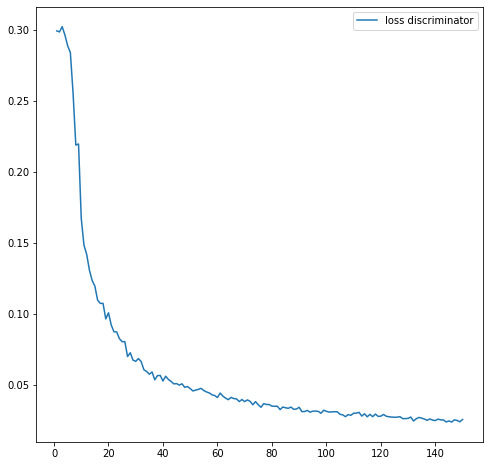
\includegraphics[width=1\linewidth]{ae_decoderXY_loss.png}
  \caption{Loss function}
  \label{subfig:ae_decoderXY_loss}
\end{subfigure}%
\begin{subfigure}{.5\textwidth}
  \centering
  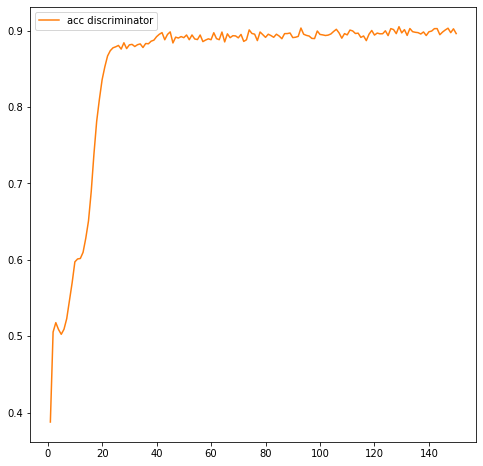
\includegraphics[width=1\linewidth]{ae_decoderXY_acc.png}
  \caption{Accuracy}
  \label{subfig:ae_decoderXY_acc}
\end{subfigure}
\caption{Training process of encoder and decoder XY}
\label{fig:ae_decoderXY}
\end{figure}

Below, results of trained models, generated for each person are presented. First column from the left contains original images to be encoded into latent vectors. Following columns present faces generated by respective decoders, from obtained feature maps. Actual deepfakes are presented in the last column, while remaining columns act as a frame of reference.

\subsection{Subject X}

\begin{figure}[H]
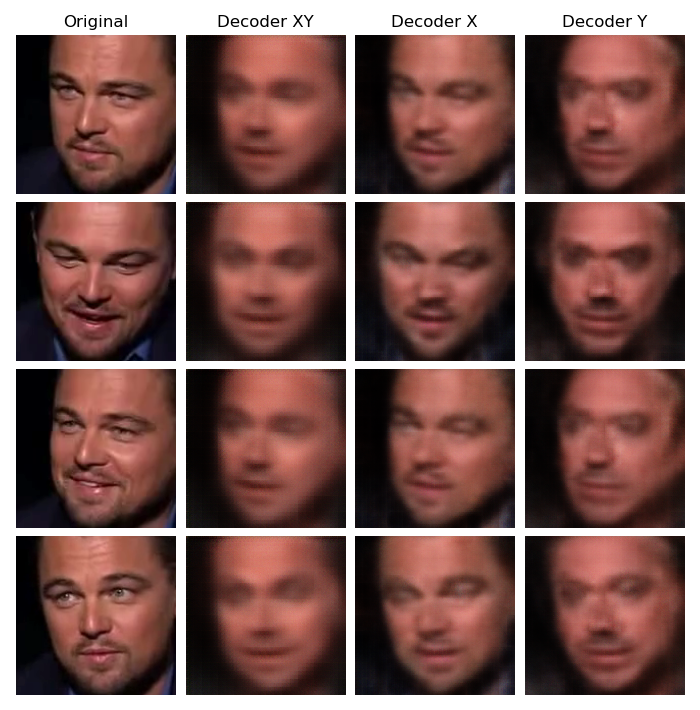
\includegraphics[width=10cm] {Results/ae_x_scene1_350.png}
\centering
\caption{Sample 1 from subject X after 350 epochs}
\label{fig:ae_x_scene1_350}
\end{figure}

\begin{figure}[H]
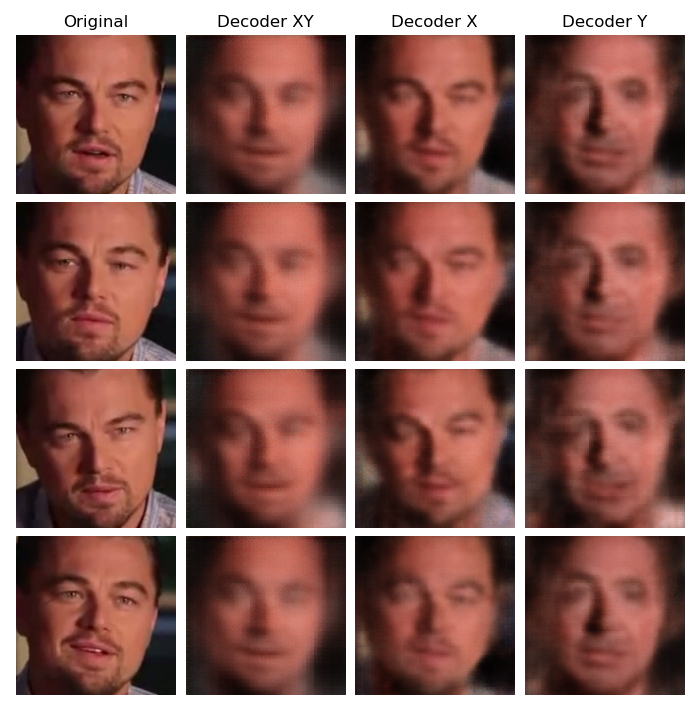
\includegraphics[width=10cm] {Results/ae_x_scene2_350.png}
\centering
\caption{Sample 2 from subject X after 350 epochs}
\label{fig:ae_x_scene2_350}
\end{figure}

\begin{figure}[H]
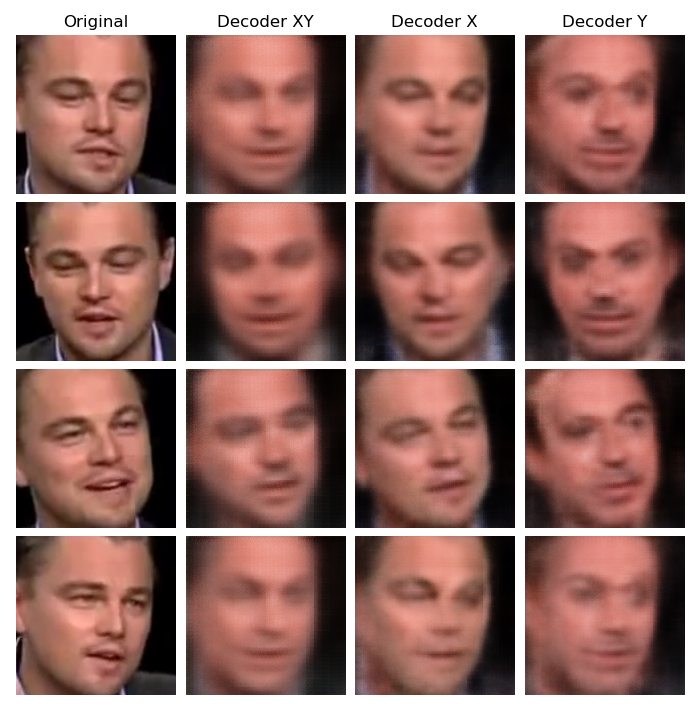
\includegraphics[width=10cm] {Results/ae_x_scene3_350.png}
\centering
\caption{Sample 3 from subject X after 350 epochs}
\label{fig:ae_x_scene3_350}
\end{figure}

\begin{figure}[H]
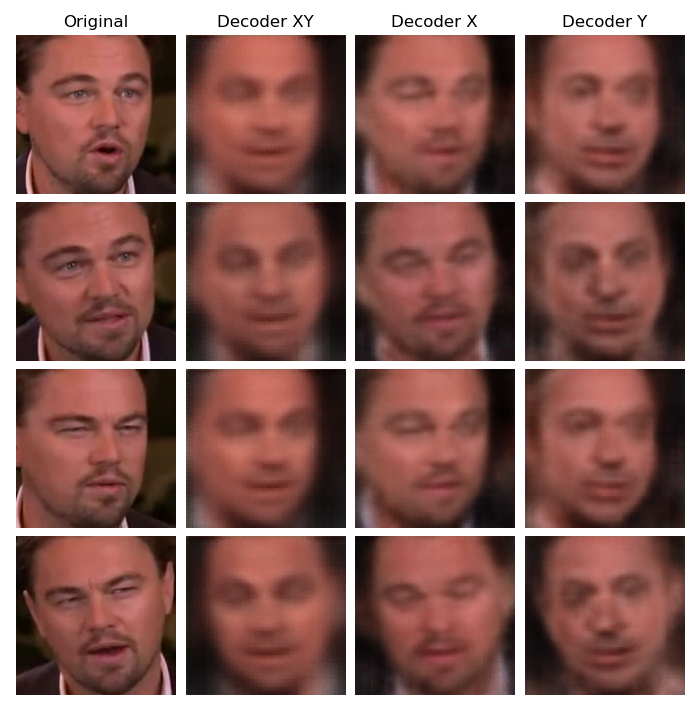
\includegraphics[width=10cm] {Results/ae_x_scene4_350.png}
\centering
\caption{Sample 4 from subject X after 350 epochs}
\label{fig:ae_x_scene4_350}
\end{figure}

\subsection{Subject Y}

\begin{figure}[H]
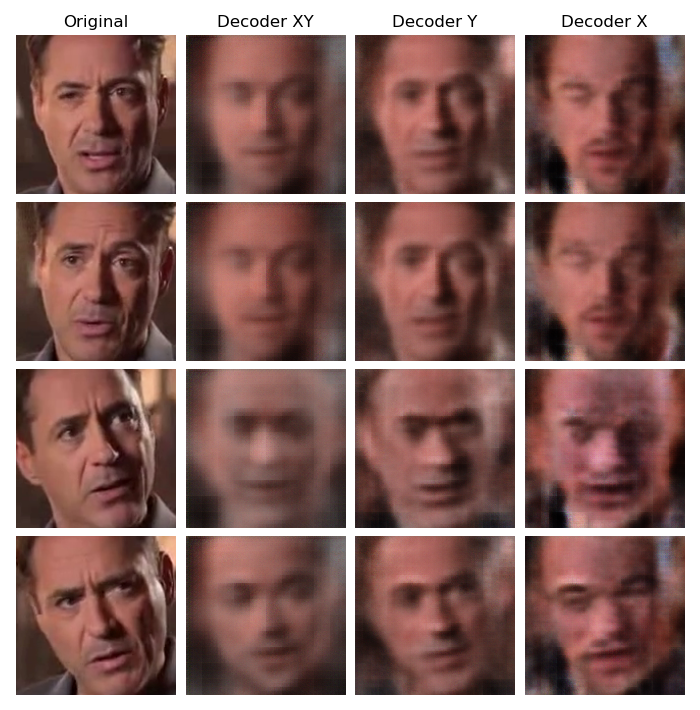
\includegraphics[width=10cm] {Results/ae_y_scene1_350.png}
\centering
\caption{Sample 1 from subject Y after 350 epochs}
\label{fig:ae_y_scene1_350}
\end{figure}

\begin{figure}[H]
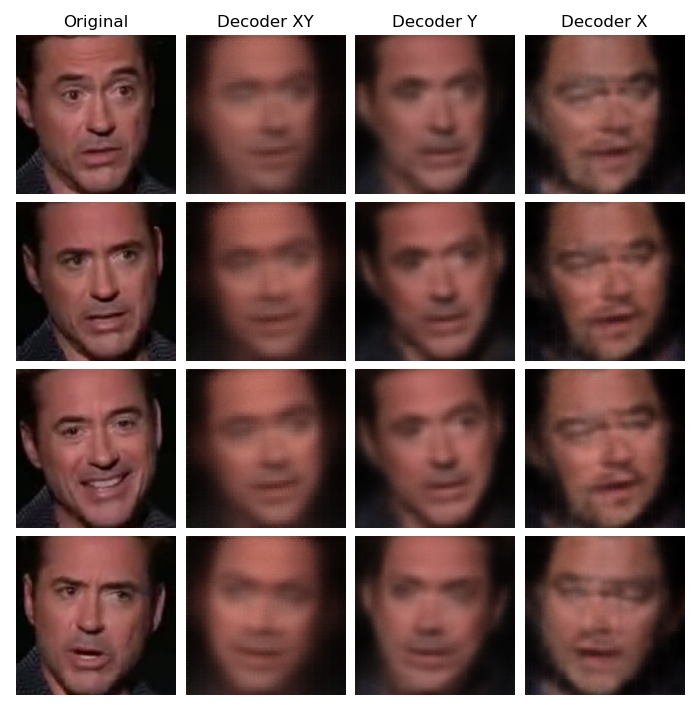
\includegraphics[width=10cm] {Results/ae_y_scene2_350.png}
\centering
\caption{Sample 2 from subject Y after 350 epochs}
\label{fig:ae_y_scene2_350}
\end{figure}

\begin{figure}[H]
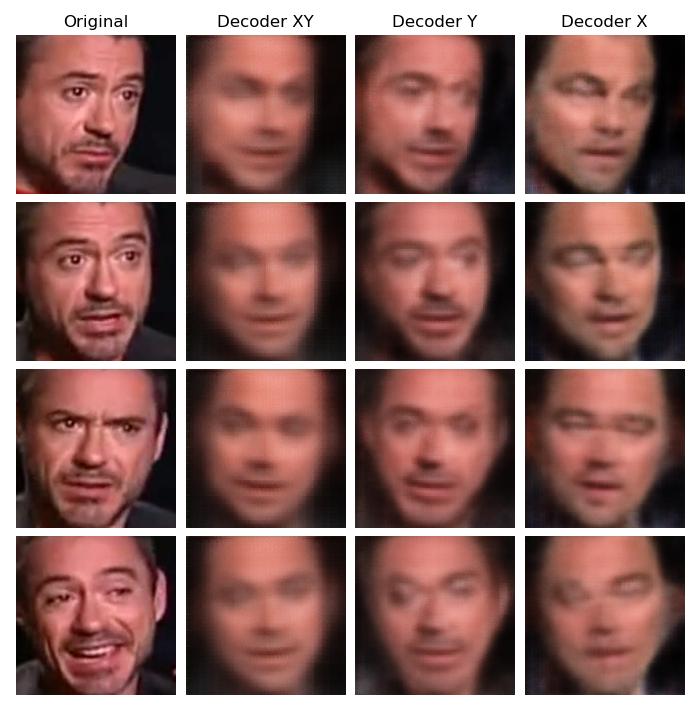
\includegraphics[width=10cm] {Results/ae_y_scene3_350.png}
\centering
\caption{Sample 3 from subject Y after 350 epochs}
\label{fig:ae_y_scene3_350}
\end{figure}

\begin{figure}[H]
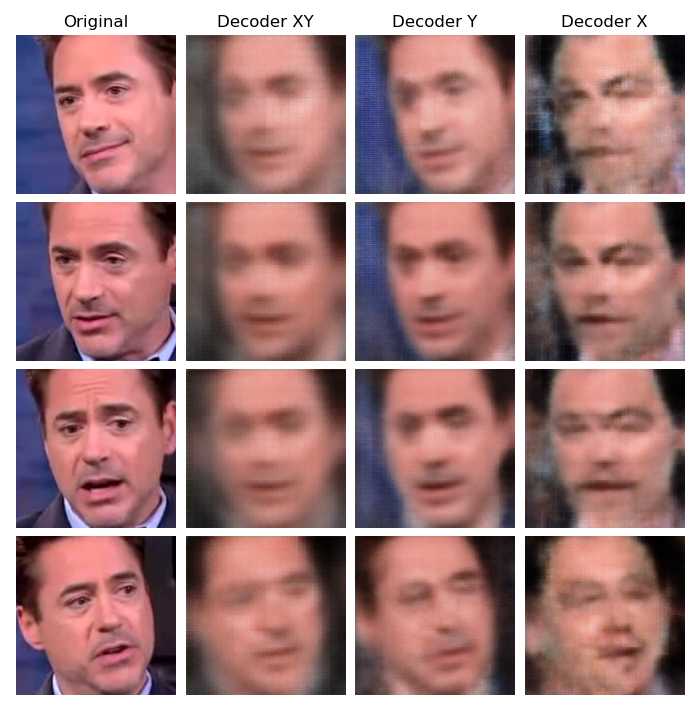
\includegraphics[width=10cm] {Results/ae_y_scene4_350.png}
\centering
\caption{Sample 4 from subject Y after 350 epochs}
\label{fig:ae_y_scene4_350}
\end{figure}

\section{Variational autoencoder}
\subsection{Subject X}
\subsection{Subject Y}
\section{VAE-GAN}
\subsection{Subject X}
\subsection{Subject Y}
\section{CycleGAN}
\subsection{Subject X}
\subsection{Subject Y}